% \section{Visualization design}
% \subsection{Query execution overview}
% \subsubsection{Execution plan view}
% \subsubsection{Execution progress view}
% \subsection{Task view}
% \subsection{System profiling visualization}
% \subsection{Linkage and interactions}

\section{Visualization design}
Following the data modeling, we present the web-based visual analytics system to support the interactive exploration with four coordinated views. The Execution progress demonstrates the overview about how the query plan are execute(\textbf{T1}), the Task distribution view shows the task distribution and the data dependencies. Integrated with the machine performance metrics, this view is also used for reason the specific patterns of tasks(\textbf{T2} and \textbf{T3}).  Task list provides the detailed information at the task level(\textbf{T2}).  At last, the interaction and linkage are introduced to support the multi-level explorations(\textbf{T4}).

\subsection{Query Progress View}\label{sec:queryprogress}


\begin{figure}[t]
	\centering
	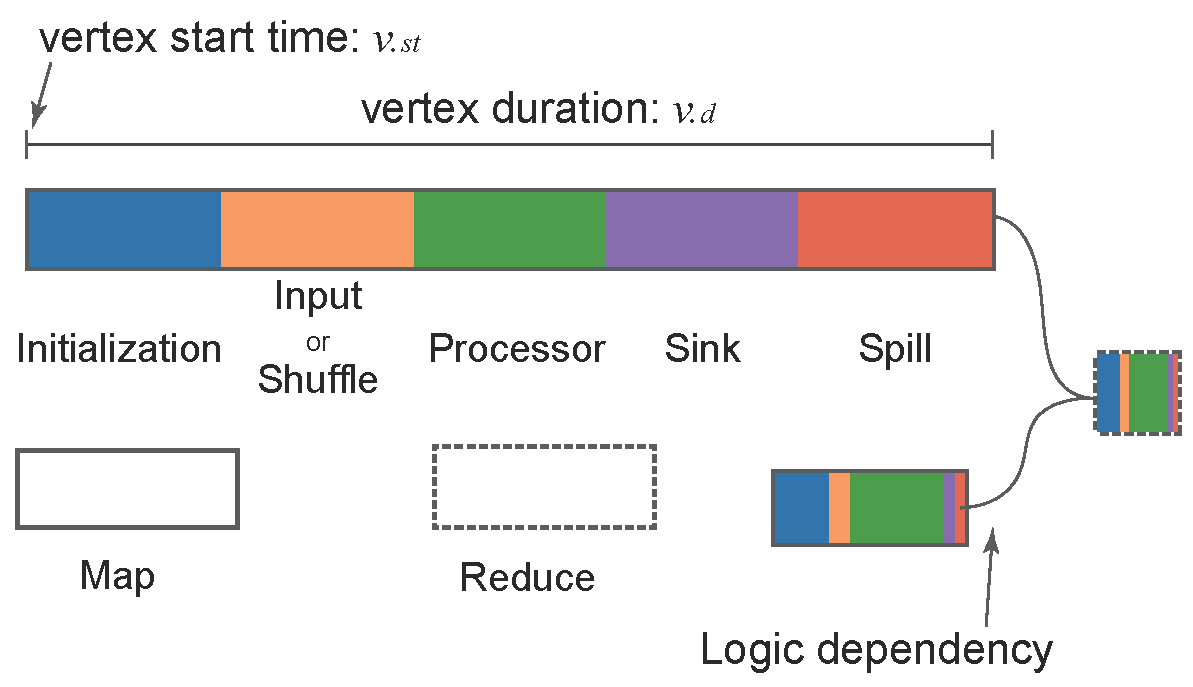
\includegraphics[width=0.35\textwidth]{figures/visualization/progressdesign.pdf}
	\vspace{-3mm}
	\caption{Visual encoding of logic vertex and dependency}
	\label{fig:progress}
	\vspace{-3mm}
\end{figure}

Query Progress View is developed to overview the overall progress of query execution and the logic dependencies. 

\begin{algorithm}
	\caption{$\mathsf{TDAGLayout}$($R$, $canvas$)}
	\label{alg:TDAGLayout}
	\begin{algorithmic}[1]
		\For {$root$ in $R$}
		\State$\mathsf{process}$($root$, $canvas$)
		\EndFor
	\end{algorithmic}

\end{algorithm}

\begin{algorithm}
	\caption{$\mathsf{process}$($v$, $canvas$)}
	\label{alg:process}
	\begin{algorithmic}[1]
		\If{$v.visit = True$}
			\State Do Nothing
		\EndIf
		\If{$v.children$ is empty}
			\If{$\mathsf{place}$($v$)$ = true $}
				\State $canvas.height \leftarrow canvas.height + uh$
				\State $\mathsf{place}$($v$)
			\EndIf
		\Else
			\For {$c$ in $v.children$}
				\State $\mathsf{process}$($c$)
				\If{$\mathsf{place}$($v$)$ = true$}
					\State $v.visit \leftarrow True$
				\EndIf
			\EndFor
			\If{$v.visit = True$}
				\State $canvas.height \leftarrow canvas.height + uh$
				\State $\mathsf{place}$($v$)
			\EndIf
		\EndIf
	\end{algorithmic}
\end{algorithm}




\subsubsection{Visual Encoding}
The commonly used method to visualize the progress data is Gantt Chart.
As shown by Figure~\ref{fig:progress}, the x-axis indicates the timestamp. The rectangles with the same height indicate the temporal information of logic vertices. 
Given a vertex $v$, the position of the left side indicates the start time $v.st$ and the duration of $v.d$ is encoded by the length of the rectangle. We use the stroke dash to present the type of vertex and use the color to encode the type of steps in a vertex. Moreover, the order of all steps is fixed as shown by Figure~\ref{fig:progress}.

\subsubsection{Layout Method}
In Gantt Diagram has been deployed to many progress visualization tools such as Tez UI and Tabula, each progress bar takes up the whole line with its left side and length encode the start time and duration, which is shown as Figure~\ref{fig:layout}(A).
Vertically, the progress bars are ordered by the start time of the vertex. In this visual design, since the layout doesn't consider the logic dependencies, it always results in a very serious cross between the links and unclear topology structure.

To tackle this problem, we design an algorithm~\ref{alg:TDAGLayout} to layout the TDAG. With an edge $e=\{u,v\}$, we define $u$ as the child of $v$ and $v$ as the parent of $u$. Moreover, we define the $root$ as the vertex which has no parents. $\mathsf{process}$ is described as Algorithm~\ref{alg:process}, which use a in-order traversal to process the vertices in the graph.  $\mathsf{place}$ is the function which tries to place the vertex in the canvas. At first, we use a naive which provides a vertex an exclusive row, which is shown as Figure~\ref{fig:layout}(B). The new layout shows a clear topology structure because the brother vertices are visited closely. However, this methods also results in a poorly using of the canvas, since some vertices can be put at the same row.  
To provide a tight layout, we revise the method $\mathsf{place}$ which tries to place the vertex at the top position of the canvas, if the vertex is overlaped with the existing vertex, then move this vertex down the distance of the vertex height. If the $\mathsf{place}$ cannot find a place for the vertex in the canvas, the $\mathsf{place}$ will return $False$ indicating the height of canvas is not enough, otherwise return $True$. Each parent vertex will be visited multiple times until it is successfully placed into the canvas(shown as line 10 to line 14). The result(Figure~\ref{fig:layout}(B)) shows a layout which requires a smaller canvas.

The tight layout further results in an unclear structure of the dependencies. We further optimized it by changing the position of the control points of B-splines. With two different source vertex, the x-position of the control points are different, thus making the lines from different source vertices are attracted to different position. The results is shown as Figure~\ref{fig:layout}(D).

\begin{figure}[t]
	\centering
	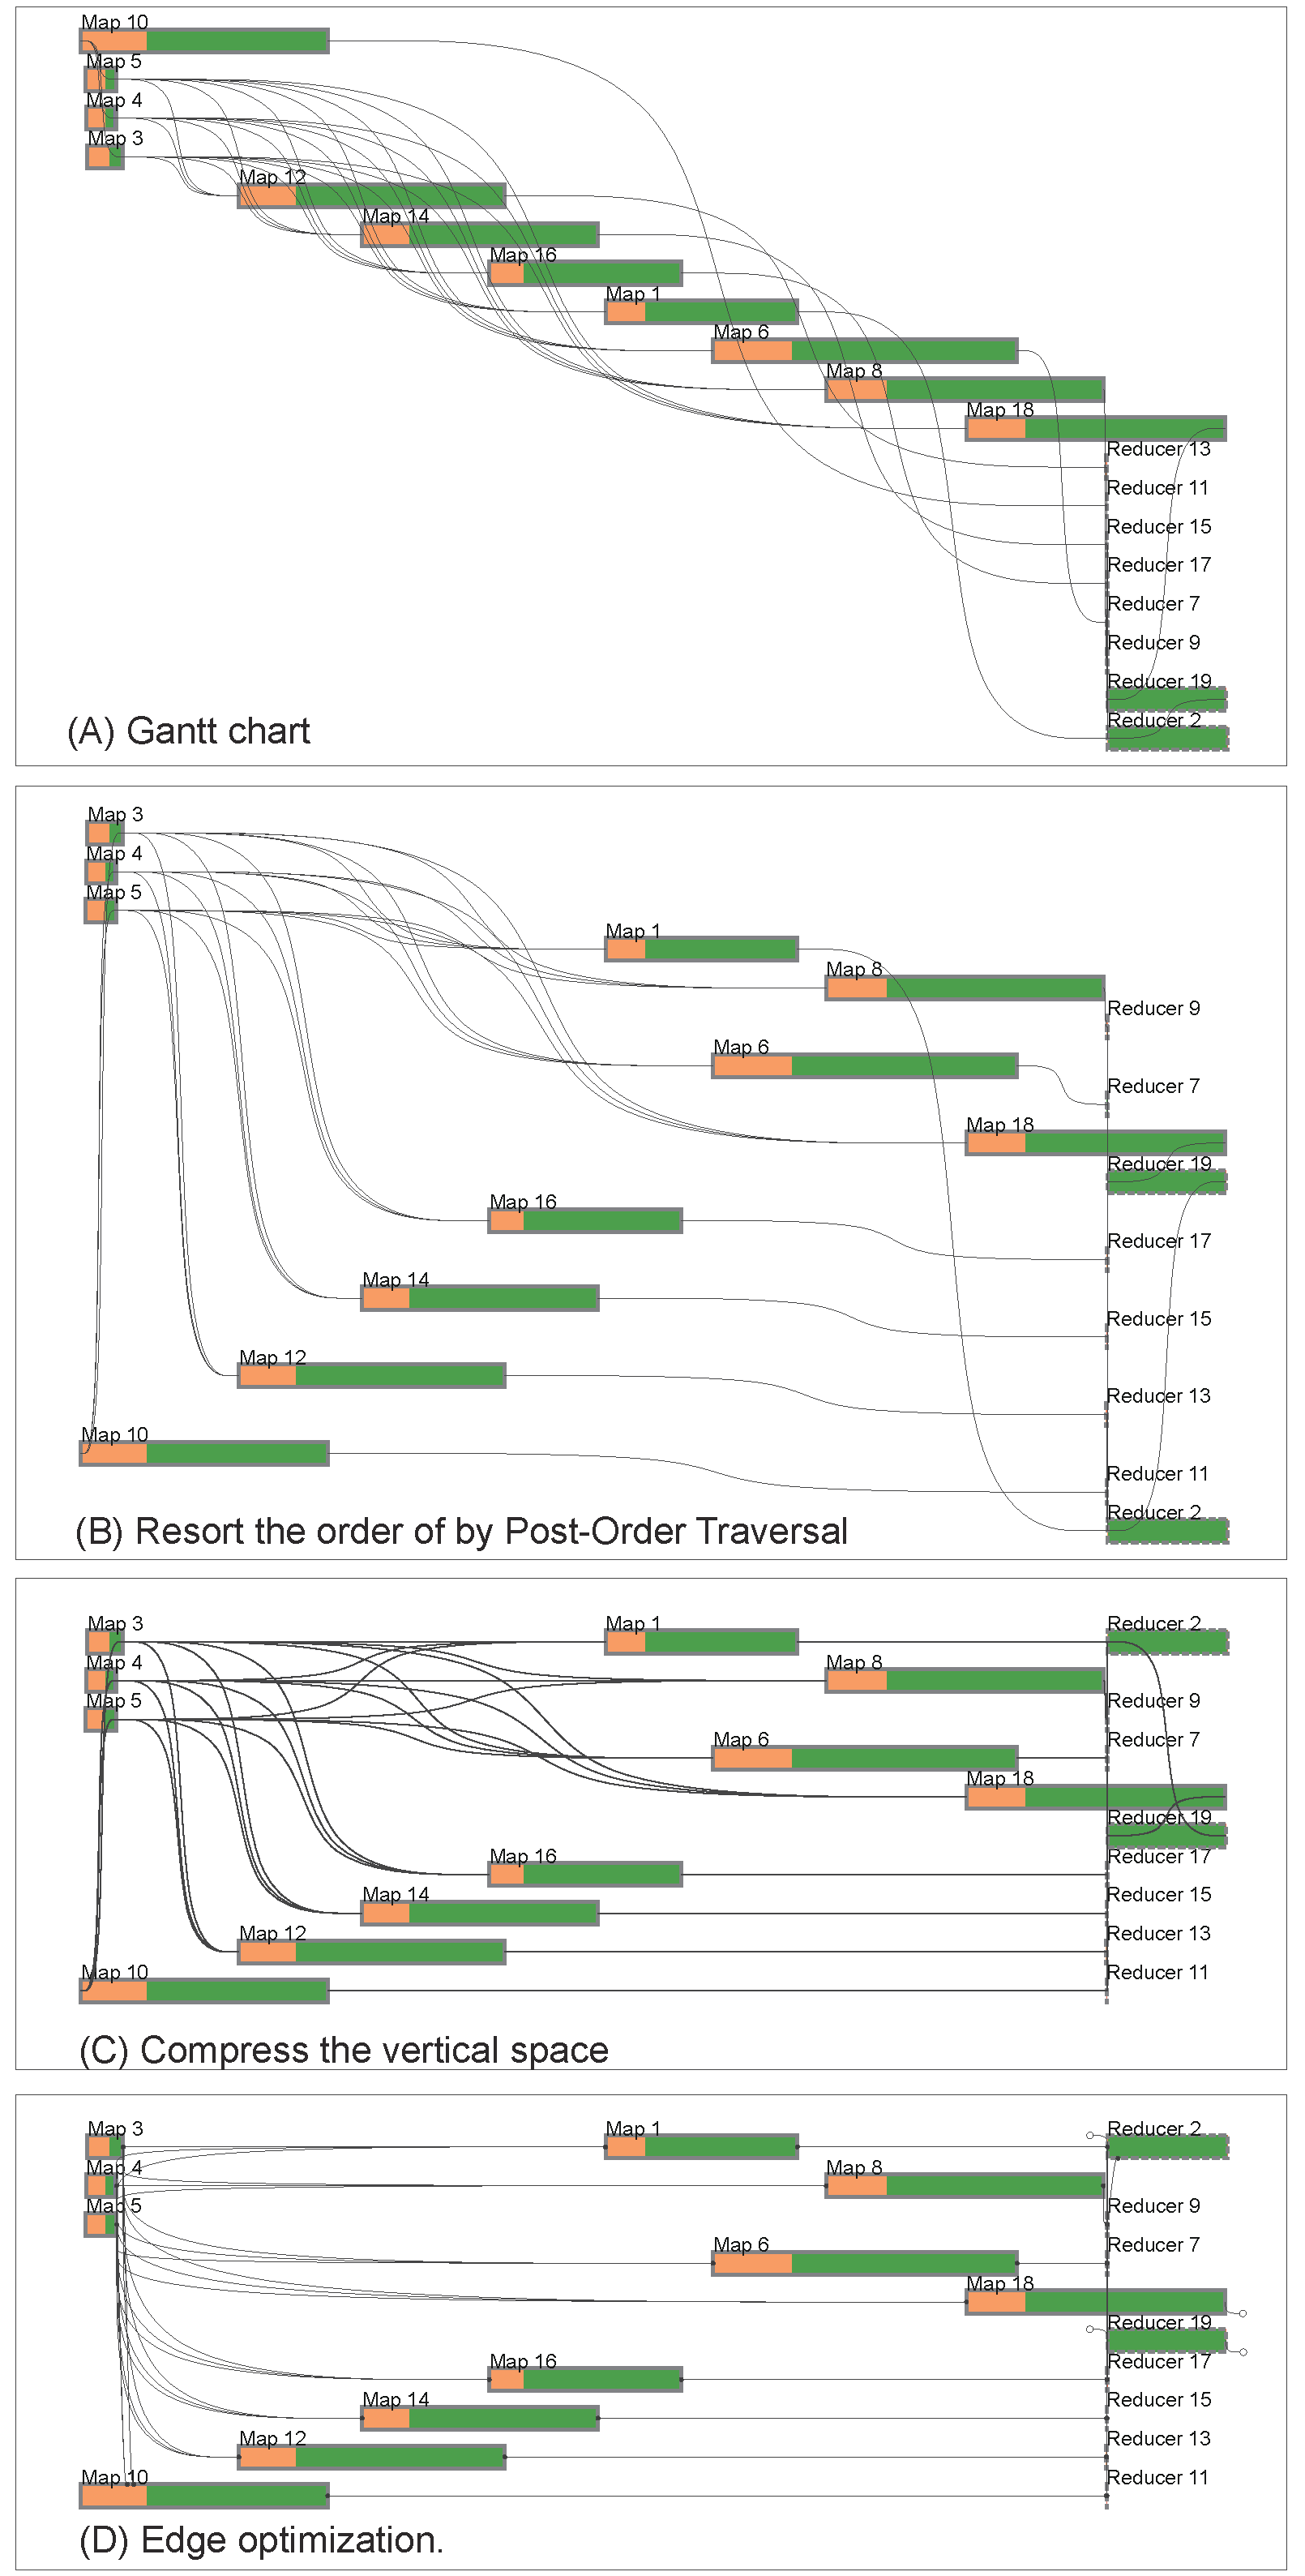
\includegraphics[width=0.45\textwidth]{figures/visualization/exeprogress.pdf}
	\vspace{-3mm}
	\caption{Temporal DAG layout algorithms}
	\label{fig:layout}
	\vspace{-3mm}
\end{figure}
%\begin{itemize}
%    \item Traditional method: Gantt diagram and design consideration 
%    \item Proposed algorithms, link processing
%    \item Alternative design
%        \begin{itemize}
%            \item Gantt(consider the vertical edge, large space, unclear structure)
%            \item New design loose(clear structure, large space)
%            \item New design compact(small space, unclear structure    )
%        \end{itemize}
%\end{itemize}

% -Visual form of Gantt diagram
% -Our design consideration
% -Algorithms
% -Design alternatives
% --gantt(consider the vertical edge, large space, unclear structure)
% --new design loose(clear structure, large space)
% --new design compact(small space, unclear structure)
% --new design compact, edge processing(small space, clear structure)
\subsection{Pattern Explorer}


\begin{figure}[t]
	\centering
	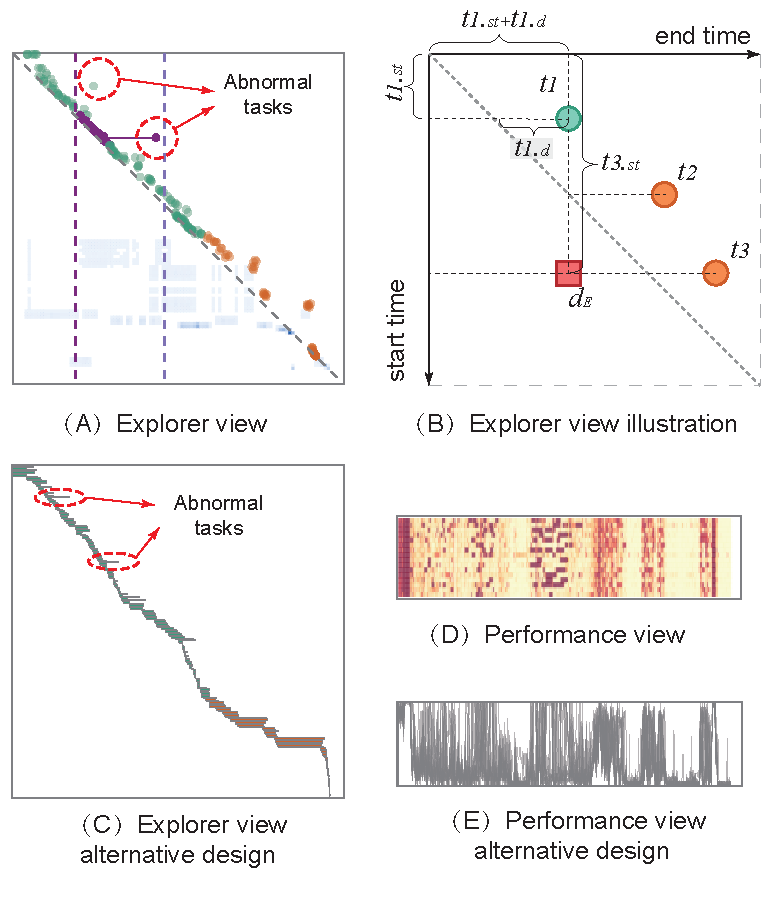
\includegraphics[width=0.48\textwidth]{figures/visualization/patternexplorer.pdf}
	\vspace{-3mm}
	\caption{Visual design for the pattern explorer.}
	\label{fig:explorer}
	\vspace{-3mm}
\end{figure}


Pattern Explorer is developed to provide efficient pattern discovery and reasoning at the task-level. This component consists of multiple coordinated views, including Distribution View and Performance View.
\subsubsection{Distribution View}
The Distribution View is designed to explore the temporal pattern and dependencies of tasks.

\stitle{Visualizing the temporal information of tasks}
Before our collaboration, the domain experts use Gantt Chart Diagram to display the overall progress of tasks, shown in figure~\ref{fig:explorer}(C). 
However, Gantt Chart Diagram-based method suffers significant scalability problem in our applications. Hundreds to thousands of tasks are associated with a vertex in our scenario, which requires a very large space to place all the horizontal bars clearly. 
Moreover, visualizing a large number of bars in this way is difficult for users to compare the absolute length of the horizontal bars due to the lack of alignment, which hinders the users' ability to discover the group-based patterns or identify the abnormal tasks.

To tackle this issue, we develop a scatter-based visual representation which is shown as Figure~\ref{fig:explorer}(A). Figure~\ref{fig:explorer}(B) illustrates the visualization design which uses a square shape of rendering canvas as the basis, the vertical axis(from top to bottom) indicates the start time, and the horizontal axis(from left to right) indicates the end time.
The task(e.g., $t_1, t_2, t_3$) with the temporal information of start time and duration can be visualized as dots layouted on the canvas. 
This design has two benefits: 1) we simplify each horizontal bars as dots. Thus the all tasks can be presented as the point cloud in the canvas. This presentation form may results in the visual clutter caused by the gathering and overlap of dots, but can significantly highlight the clusters and outliers, which can help the users to find the task of interest; 2) we linearly map the time range to both horizontal and vertical axis. In this way, as shown by task $t_1$ in figure~\ref{fig:explorer}(B) the horizontal distance from point to the diagonal line of canvas represents the duration(e.g., $t_2.d$) of the task, which helps the users to \QM{compare the task duration}. Generally speaking, in this view, if a task has a long duration, it tends to move to the top right corner. 

We compare our design with Gantt Chart shown as ~\ref{fig:explorer}(C), we scale the height of the bars of Gantt Chart to visualize the all tasks in the view with same size of our design. It is found that in our design, the outliers are more easily observed and the overall temporal distribution is more clear in our design than Gantt Chart.

\stitle{Visualizing the task dependencies} 
The direct way to visualize the data dependencies is to use the curves such as the Query Progress View(section~\ref{sec:queryprogress}). However, such design will result in a serious visual clutter when dealing with the large data size. To solve this problem, we also transform the dependencies as a dot on the render canvas. As shown by Figure~\ref{fig:explorer}(B), the dependency $d_E$ from task $t_1$ to $t_3$ is visualized as a dot(red color rectangle) in the left bottom part of canvas, which presents the end time or producer task and the start time of consumer task.  To further deal with the scalability problem, we use heatmap instead of point cloud to improve the render efficiencies.

This design utilizes the left half part of canvas and showing the distribution of dependencies according to their temporal information, allowing the users to discover the long dependency duration clusters. 

To facility the interactive explorations, several interactions are implemented in this view. For example, once a task is selected, the corresponding dependencies will be highlighted on the canvas as individual points, which is shown as ~\ref{}. Moreover, users can select the time range of interest by brush the a timeline at the horizontal or vertical boundaries of canvas,then the time range of this view will be updated to allow users to switch their focus. Moreover, when the users select a vertex, the associated tasks will be highlighted in purple color, which is shown as Figure~\ref{}.

\stitle{Visualizing system performance metrics}
As introduced in section~\ref{sec:systemdesign}, several metrics affecting the query performance are collected. These metrics can be modeled as multi-dimensional time-series data. For example, a machine may have 12 CPUs, thus the usage of the CPU can be modeled as a temporal sequence with 12 dimensions. We use the heatmap-based visualization to demonstrate temporal trend of CPUs(shown as Figure~\ref{fig:explorer}(D)). We use the color range from yellow to red to encode the CPU usage from 0 to 100$\%$. Another visualization form for the multi-dimensional time-series data is linechart, which can provide more accurate visualization than color encoding when the dimension number is small. But when we use linechart to show the CPU usage(shown as Figure~\ref{fig:explorer}(E)), the lines results in a serious visual clutter which cannot deliver useful information at all. For all the machine metrics, CPU usage and Disk information both contains more than 10 dimensions, which we use heatmap-based visualization. For other metrics such Memory and Network, the number of dimensions is less than five and we use the linechart as the visualization methods. To support the correlation discovery between the patterns in task distribution and system performance metrics, we set the same time scale for both the task distribution view and performance metric view.

 
% \begin{itemize}
%     \item Design consideration. Why gantt doesn't work(need very large space, difficult to show the data-flow link, difficult to show and select the abnormal cases)
%     \item Our design
%     \item Compare with design alternative (Gantt)
% \end{itemize}


\subsection{Task List View}


\begin{figure}[t]
	\centering
	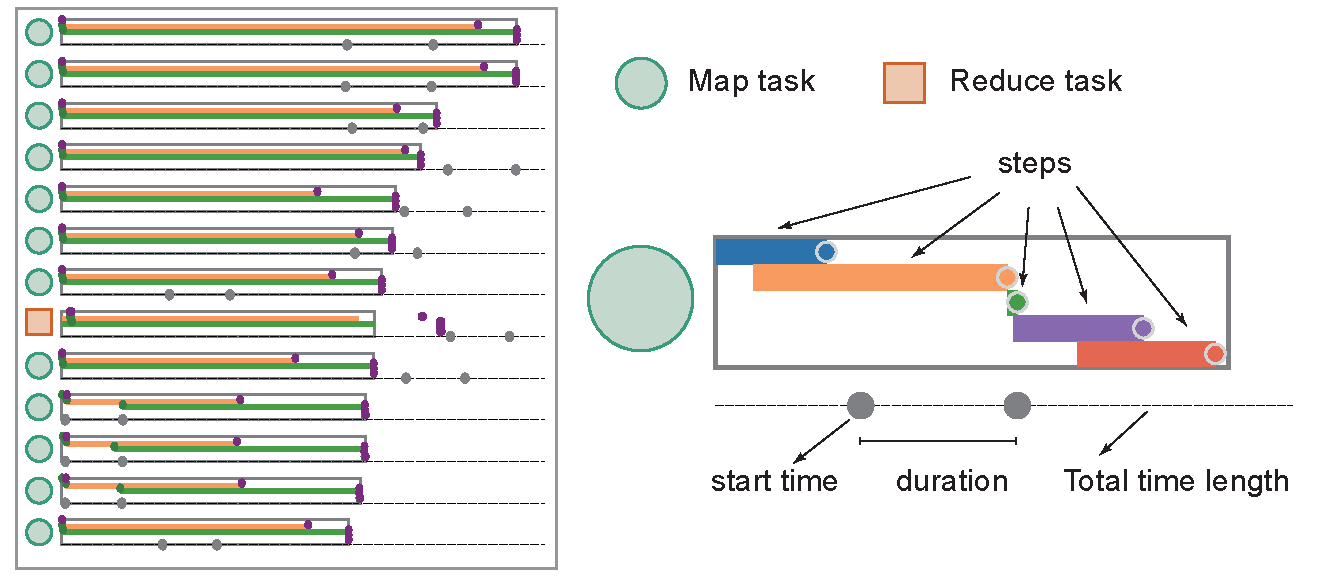
\includegraphics[width=0.48\textwidth]{figures/visualization/taskList.pdf}
	\vspace{-3mm}
	\caption{Visual design for task list.}
	\label{fig:taskList}
	\vspace{-3mm}
\end{figure}

Task list view is developed to enable the detailed exploration of the individual tasks.
All the tasks will be listed from the top to the bottom according to the duration, and only the top one hundred tasks are shown by default.There are two visual forms of a task: glyph form and extension form. By default, the task glyph are placed row by row. When the user select the task of interest, the glyph will be extended as the extension form(shown as ~\ref{**}).


\subsubsection{Task glyph}
As shown by Figure~\ref{fig:taskList}, the green circle or orange rectangle is placed at the left side of a row, indicating the type of the task. On the right side, a rectangle is shown with the length to encode the relative task duration to the maximum duration for all tasks. In the rectangle, the five steps are shown line by line. We use both the color and the y-position to encode the step type. Moreover, the length of a step can be very close to 0, which makes the current visualization unobservable. To tackle this problem, we place a circle and a triangle at the left and right sides of the rectangle of a step, respectively. Thus, the zero-length step will be marked by the overlap of the two shapes.

\subsubsection{Extension View}
When the user clicks the task, an extension view is displayed below to the task glyph, shown as Figure~\ref{fig:taskList}(\textbf{XX}). There are two sub-components in this view: abnormal component and dependency component. 


We first conduct the abnormal detection for the tasks. As suggested by the domain experts, a task is abnormal when its duration is significantly longer than that of other tasks associated with the same vertex and executed on the same machine. Based on these suggestions, we use Tukey Fence~\cite{tukey1977exploratory} to decide if a task is abnormal. With a given set of real integer $S$ and $l \in S$, the anomaly is calculated as follows:

\begin{equation} 
AB(l, S) = \left \{
  \begin{aligned}
    &true, && \text{if}\ l > S.q_3+1.5(S.q_3-S.q_1)\\
    &false, && \text{otherwise}
  \end{aligned} \right.
\end{equation}

Where $S.q_i$ is the $i^{th}$ quartile of set $S$. With the given task and the vertex, we conduct the abnormal detection for the duration of the task and each step. 

After calculation, we design the abnormal component with six rows. With a given vertex $v$ and the task $t$. The top fives row visualize the distribution of the five steps in $v$ as boxplot: the left and right vertical lines indicate the minimum and maximum duration of corresponding steps, and the left and right sides of the rectangle indicate the $1^{st}$ and $3^{st}$ quartiles. We also place a dot over the boxplot to show the duration of task $t$. The last row is implemented to use the same visual form which is used for the presentation of task duration.

The dependency components consists two rows representing the producer tasks and the consumer tasks respectively. With a given task, the number of its consumer tasks and producer tasks may reach thousands of tasks. Considering the scalability issues, we use the pixel barchart~\cite{keim2002pixel} to visualize data amount of dependencies. For example, as shown in Figure~\ref{fig:explorer}{(XX)}, we vertically divide the dependency component into segments to present the machines. 
The consumer tasks or producer tasks are visualized as the pixels in machine box execute this task, the position of task is decided by the data size transmit between the tasks, which is layouted from left to right and from top to bottom. The color is also used to encode the data size. 



%\begin{itemize}
%    \item Our design consideration
%    \item Design: Embedding task view to profiling view
%    \item Design: Visualize the profiling results
%\end{itemize}

\subsection{Interactions}
To facilitate the interactive exploration, out system supports the cross-view interactions. 
In summary, there are two categories of interactions are implemented in the system: cross-level interactions and temporal linkage.

\stitle{Cross-level and -view interactions}:
Our system supports linking among visual elements related to the same task. 
For example, when hovering the mouse on the task of Task View, the corresponding dots of this task and the data dependencies at the machine view will be highlighted by changing the color to purple. Moreover, the progress bar of vertex associated with the task will also be highlighted by change the stroke width.   

\stitle{Temporal linkage}
In both machine view and progress view allow, users can select the time range to narrow down to the pattern of interest. When select time range at any view, the time focus of other views will be updated. 
%    \item Multi-scale navigation
%    \item Inner and inter linking
%\end{itemize}
